\chapter{Solutions and Solubility}\label{ch:g6:solutions-and-solubility}

A bottle of sparkling water is opened: a hiss, and a rush of tiny bubbles
rises from nowhere. The water looked perfectly clear a second earlier,
yet a gas was dissolved in it all along. Solids \omterm{def:g2:mixing-and-dissolving:dissolve}{dissolve}, liquids
\omterm{def:g2:mixing-and-dissolving:dissolve}{dissolve}, and gases \omterm{def:g2:mixing-and-dissolving:dissolve}{dissolve} too --- but never without limit. This
chapter names the parts of a solution and measures how much of a
substance a liquid can hold.

\begin{recall}
A solid that \omterm{def:g2:mixing-and-dissolving:dissolve}{dissolves} in water disappears from sight and leaves the
liquid clear; the clear liquid is a solution, and what was dissolved is
still in it (\cref{ch:g2:mixing-and-dissolving}). A solution is a
\omterm{def:g6:pure-substances-and-mixtures:homogeneous}{homogeneous mixture} of \omterm{def:g6:pure-substances-and-mixtures:species}{chemical species}
(\cref{ch:g6:pure-substances-and-mixtures}). \omterm{def:g3:separating-mixtures:evaporate}{Evaporating} the water gets
the dissolved solid back (\cref{ch:g3:separating-mixtures}).
\end{recall}

\begin{omfigure}
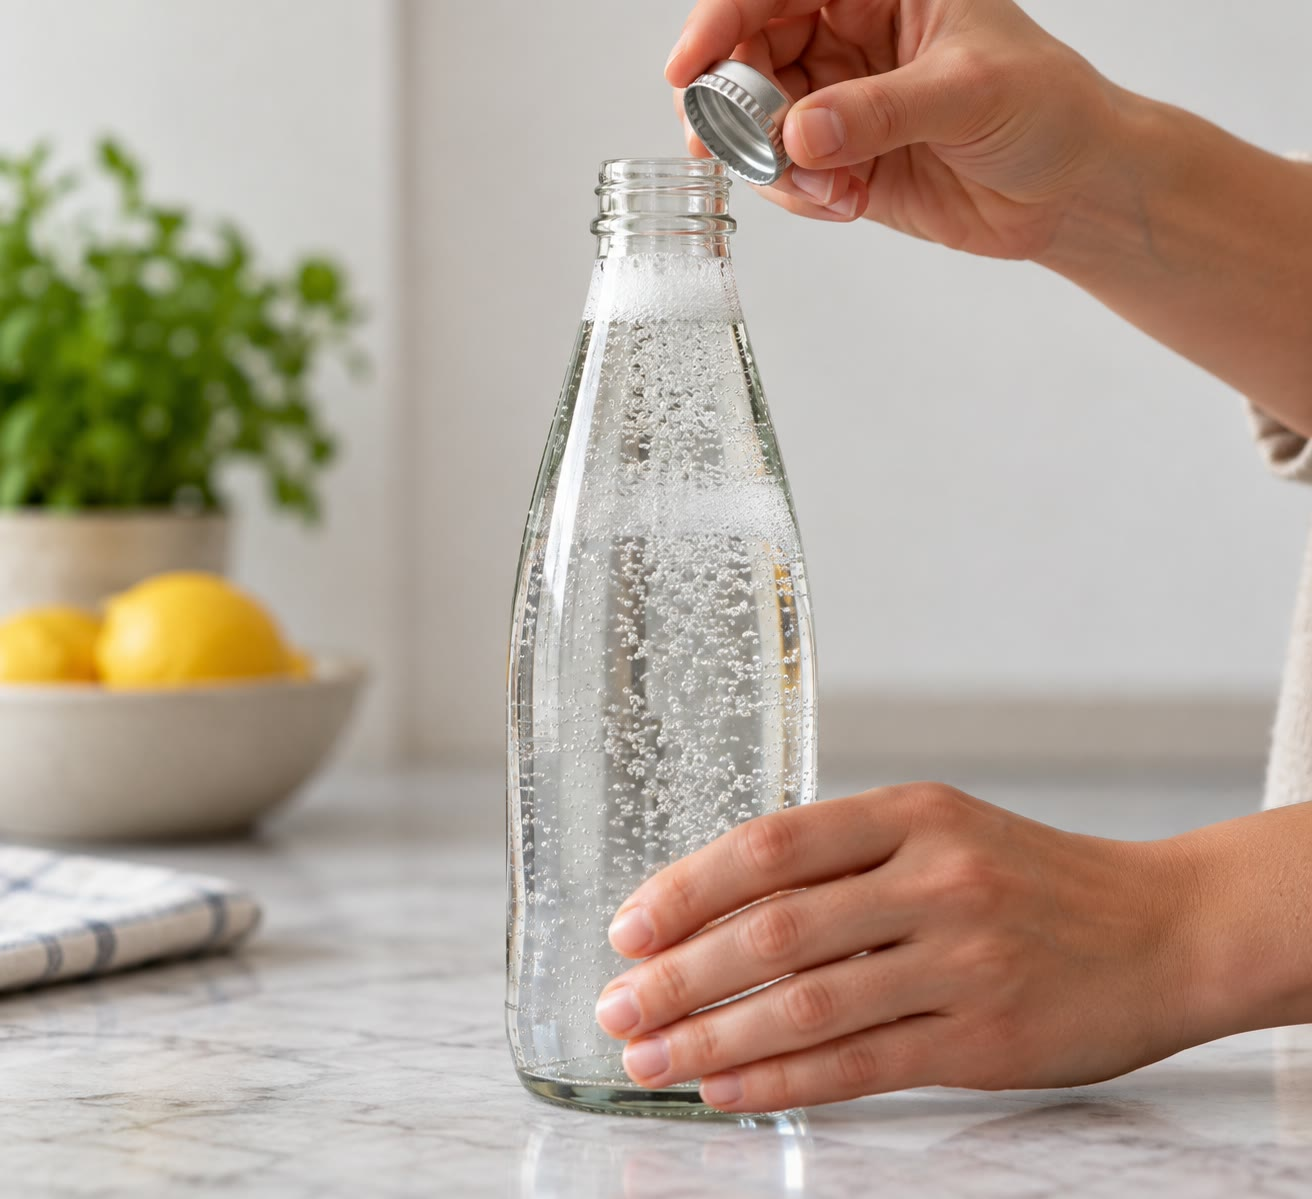
\includegraphics[width=0.5\linewidth]{images/book1/ai/g6-fizzy-water.jpg}

{\small Opening a bottle of sparkling water: the dissolved gas comes out
as bubbles.}
\end{omfigure}

\section{Solute and solvent}

\begin{definition}[Solute, solvent, aqueous solution]\label{def:g6:solutions-and-solubility:solute}
In a solution, the substance that \omterm{def:g2:mixing-and-dissolving:dissolve}{dissolves} is the
\emph{solute}\index{solute}, and the liquid it \omterm{def:g2:mixing-and-dissolving:dissolve}{dissolves} in is the
\emph{solvent}\index{solvent}. When the solvent is water, the solution
is an \emph{aqueous solution}\index{aqueous solution}.
\end{definition}

\begin{example}[Solvents other than water]\label{ex:g6:solutions-and-solubility:solvents}
Water is the commonest \omterm{def:g6:solutions-and-solubility:solute}{solvent}, but not the only one. Nail varnish does
not \omterm{def:g2:mixing-and-dissolving:dissolve}{dissolve} in water; it \omterm{def:g2:mixing-and-dissolving:dissolve}{dissolves} in propanone (acetone), the \omterm{def:g6:solutions-and-solubility:solute}{solvent}
of nail-varnish remover. Grease and oil paint \omterm{def:g2:mixing-and-dissolving:dissolve}{dissolve} in white spirit.
Many medicines are dissolved in ethanol. A solution can have several
\omterm{def:g6:solutions-and-solubility:solute}{solutes}: sea water holds dissolved salt and many other substances.
\end{example}

\begin{safety}{\ghs{GHS02}\ghs{GHS07}}
% ledger: ghs:acetone
Propanone (acetone): highly flammable liquid and vapour (GHS02); it
irritates the eyes and its vapour can make one drowsy or dizzy (GHS07).
It is used in a ventilated room, far from any flame.
\end{safety}

\begin{proposition}[The masses add up]\label{prop:g6:solutions-and-solubility:mass}
The mass of a solution is the mass of the \omterm{def:g6:solutions-and-solubility:solute}{solvent} plus the mass of the
dissolved \omterm{def:g6:solutions-and-solubility:solute}{solute}: nothing is lost when a solid \omterm{def:g2:mixing-and-dissolving:dissolve}{dissolves}, even though it
can no longer be seen.
\end{proposition}

\begin{omfigure}
\begin{tikzpicture}[font=\small, scale=1.15]
  \pic[transform shape] at (0,0) {balance};
  \pic[transform shape] at (0,0.8) {beaker={0.5}{omWater!80}};
  \node[anchor=north, align=center] at (0,-0.1) {\qty{100}{g} of water};
  \node at (1.85,1.3) {$+$};
  \pic[transform shape] at (3.5,0) {balance};
  \fill[white, draw=black!45] (3.0,0.8) rectangle (4.0,0.9);
  \fill[white, draw=black!45] (3.15,0.9) -- (3.85,0.9) -- (3.5,1.2) -- cycle;
  \node[anchor=north, align=center] at (3.5,-0.1) {\qty{10}{g} of sugar};
  \draw[->, thick, omProp] (4.9,1.2) -- (6.0,1.2) node[midway, above, text=black]
    {stir};
  \pic[transform shape] at (7.4,0) {balance};
  \pic[transform shape] at (7.4,0.8) {beaker={0.52}{omWater!80}};
  \node[anchor=north, align=center] at (7.4,-0.1) {\qty{110}{g} of sugar water};
\end{tikzpicture}

{\small Dissolving \qty{10}{g} of sugar in \qty{100}{g} of water gives
\qty{110}{g} of solution (the mass of the beaker is left out).}
\end{omfigure}

\section{Saturation and solubility}

\begin{definition}[Saturated solution]\label{def:g6:solutions-and-solubility:saturated}
A solution is a \emph{saturated solution}\index{saturated solution} when
it cannot \omterm{def:g2:mixing-and-dissolving:dissolve}{dissolve} any more of its \omterm{def:g6:solutions-and-solubility:solute}{solute}: any \omterm{def:g6:solutions-and-solubility:solute}{solute} added stays at the
bottom, undissolved, however long we stir.
\end{definition}

\begin{definition}[Solubility]\label{def:g6:solutions-and-solubility:solubility}
The \emph{solubility}\index{solubility} of a \omterm{def:g6:solutions-and-solubility:solute}{solute} in a \omterm{def:g6:solutions-and-solubility:solute}{solvent} is the
largest mass of \omterm{def:g6:solutions-and-solubility:solute}{solute} that a given amount of \omterm{def:g6:solutions-and-solubility:solute}{solvent} can \omterm{def:g2:mixing-and-dissolving:dissolve}{dissolve}, at a
given temperature. For a solid in water it is often given in grams per
litre (or per kilogram) of water.
\end{definition}

\begin{proposition}[Some solubilities in water]\label{prop:g6:solutions-and-solubility:values}
% ledger: sol:NaCl, sol:sucrose, sol:CO2, sol:O2 (O2: 31 mL/L, 31/24.0 x 32 = 0.041 g/L at 20 C)
Measured solubilities in water differ enormously:
\begin{center}
\small
\begin{tabular}{lll}
\hline
\omterm{def:g6:solutions-and-solubility:solute}{solute} & \omterm{def:g6:solutions-and-solubility:solubility}{solubility} in water & conditions \\
\hline
sugar (sucrose) & about \qty{2000}{g} per litre of water & room temperature \\
salt (sodium chloride) & \qty{360}{g} per kilogram of water & \qty{25}{\celsius} \\
carbon dioxide & about \qty{1.5}{g} per litre & \qty{25}{\celsius}, under the gas \\
oxygen & about \qty{0.04}{g} per litre & \qty{20}{\celsius}, under the gas \\
sand, chalk & practically none & --- \\
\hline
\end{tabular}
\end{center}
A litre of water can \omterm{def:g2:mixing-and-dissolving:dissolve}{dissolve} more than its own mass of sugar, but
not even half a gram of oxygen.
\end{proposition}

\begin{method}[Will it all dissolve?]\label{met:g6:solutions-and-solubility:will-it}
To know whether a mass $m$ of \omterm{def:g6:solutions-and-solubility:solute}{solute} \omterm{def:g2:mixing-and-dissolving:dissolve}{dissolves} completely in a volume of
water:
\begin{enumerate}
  \item find the \omterm{def:g6:solutions-and-solubility:solubility}{solubility} of the \omterm{def:g6:solutions-and-solubility:solute}{solute} (in g per litre of water);
  \item compute the largest mass that this volume of water can \omterm{def:g2:mixing-and-dissolving:dissolve}{dissolve};
  \item compare with $m$: if $m$ is smaller, everything \omterm{def:g2:mixing-and-dissolving:dissolve}{dissolves}; if $m$
        is larger, the solution is saturated and the rest stays at the
        bottom.
\end{enumerate}
\end{method}

\begin{example}[Salt in a glass]\label{ex:g6:solutions-and-solubility:glass}
% ledger: sol:NaCl
Can \qty{50}{g} of salt \omterm{def:g2:mixing-and-dissolving:dissolve}{dissolve} in \qty{200}{mL} of water (about
\qty{200}{g})? One kilogram of water \omterm{def:g2:mixing-and-dissolving:dissolve}{dissolves} at most \qty{360}{g} of
salt, so \qty{200}{g} of water \omterm{def:g2:mixing-and-dissolving:dissolve}{dissolves} at most $360 \times
\frac{200}{1000} = \qty{72}{g}$. Since $50 < 72$, all the salt
\omterm{def:g2:mixing-and-dissolving:dissolve}{dissolves}.
\end{example}

\begin{omfigure}
\begin{tikzpicture}[font=\small, scale=1.15]
  \pic[transform shape] at (0,0) {beaker={0.6}{omWater!80}};
  \node[anchor=north, align=center] at (0,-0.15) {a little salt:\\ all dissolved};
  \pic[transform shape] at (3.2,0) {beaker={0.6}{omWater!80}};
  \node[anchor=north, align=center] at (3.2,-0.15) {more salt:\\ just saturated};
  \pic[transform shape] at (6.4,0) {beaker={0.6}{omWater!80}};
  \fill[black!12, draw=black!50] (5.7,0) -- (7.1,0) -- (6.9,0.2) -- (5.9,0.2) -- cycle;
  \foreach \x in {5.85,6.05,6.25,6.45,6.65,6.85} \fill[black!45] (\x,0.09) circle (0.03);
  \node[anchor=north, align=center] at (6.4,-0.15) {too much salt:\\ the rest stays undissolved};
\end{tikzpicture}

{\small Adding more and more salt to the same water. Once the solution is
saturated, extra salt stays at the bottom.}
\end{omfigure}

\begin{inthelab}[Saturating salt water]
The teacher adds salt to \qty{100}{mL} of water one spoonful at a time,
stirring well after each. The first spoonfuls disappear; then a
spoonful no longer \omterm{def:g2:mixing-and-dissolving:dissolve}{dissolves} completely and white grains stay at the
bottom: the solution is saturated. Weighing the salt used shows that
about \qty{36}{g} have dissolved.
\end{inthelab}

\section{Miscible and immiscible liquids}

\begin{definition}[Miscible and immiscible liquids]\label{def:g6:solutions-and-solubility:miscible}
Two liquids are \emph{miscible}\index{miscible} when, mixed together,
they give one single homogeneous liquid. They are
\emph{immiscible}\index{immiscible} when they separate into two layers,
the lighter one on top.
\end{definition}

\begin{example}[Water with ethanol, water with oil]\label{ex:g6:solutions-and-solubility:liquids}
Water and ethanol are \omterm{def:g6:solutions-and-solubility:miscible}{miscible}: shaken together, they give one clear
liquid. Water and oil are \omterm{def:g6:solutions-and-solubility:miscible}{immiscible}: however hard they are shaken, the
oil comes back up and floats on the water in a separate layer. In a jar
of salad dressing the oil floats above the vinegar, which is mostly
water.
\end{example}

\begin{omfigure}
\begin{tikzpicture}[font=\small, scale=1.3]
  \pic[transform shape] at (0,0) {testtube={0.6}{omWater!80}};
  \node[anchor=north, align=center] at (0,-0.15) {water + ethanol:\\ one layer};
  \pic[transform shape] at (3,0) {testtube={0.65}{yellow!55!orange!60}};
  \begin{scope}
    \clip (2.75,3) -- (2.75,0.25) arc[start angle=180, end angle=360, radius=0.25]
      -- (3.25,3) -- cycle;
    \fill[omWater!80] (2.7,0) rectangle (3.3,1.1);
  \end{scope}
  \draw[omGlass, line width=0.7pt] (2.75,3) -- (2.75,0.25) arc[start angle=180,
    end angle=360, radius=0.25] -- (3.25,3);
  \draw[<-, omProp, thick] (3.3,1.55) -- (4.1,1.75) node[right, text=black] {oil};
  \draw[<-, omProp, thick] (3.3,0.6) -- (4.1,0.6) node[right, text=black] {water};
  \node[anchor=north, align=center] at (3,-0.15) {water + oil:\\ two layers};
\end{tikzpicture}

{\small \omterm{def:g6:solutions-and-solubility:miscible}{Miscible} liquids give one layer; \omterm{def:g6:solutions-and-solubility:miscible}{immiscible} liquids give two.}
\end{omfigure}

\begin{omfigure}
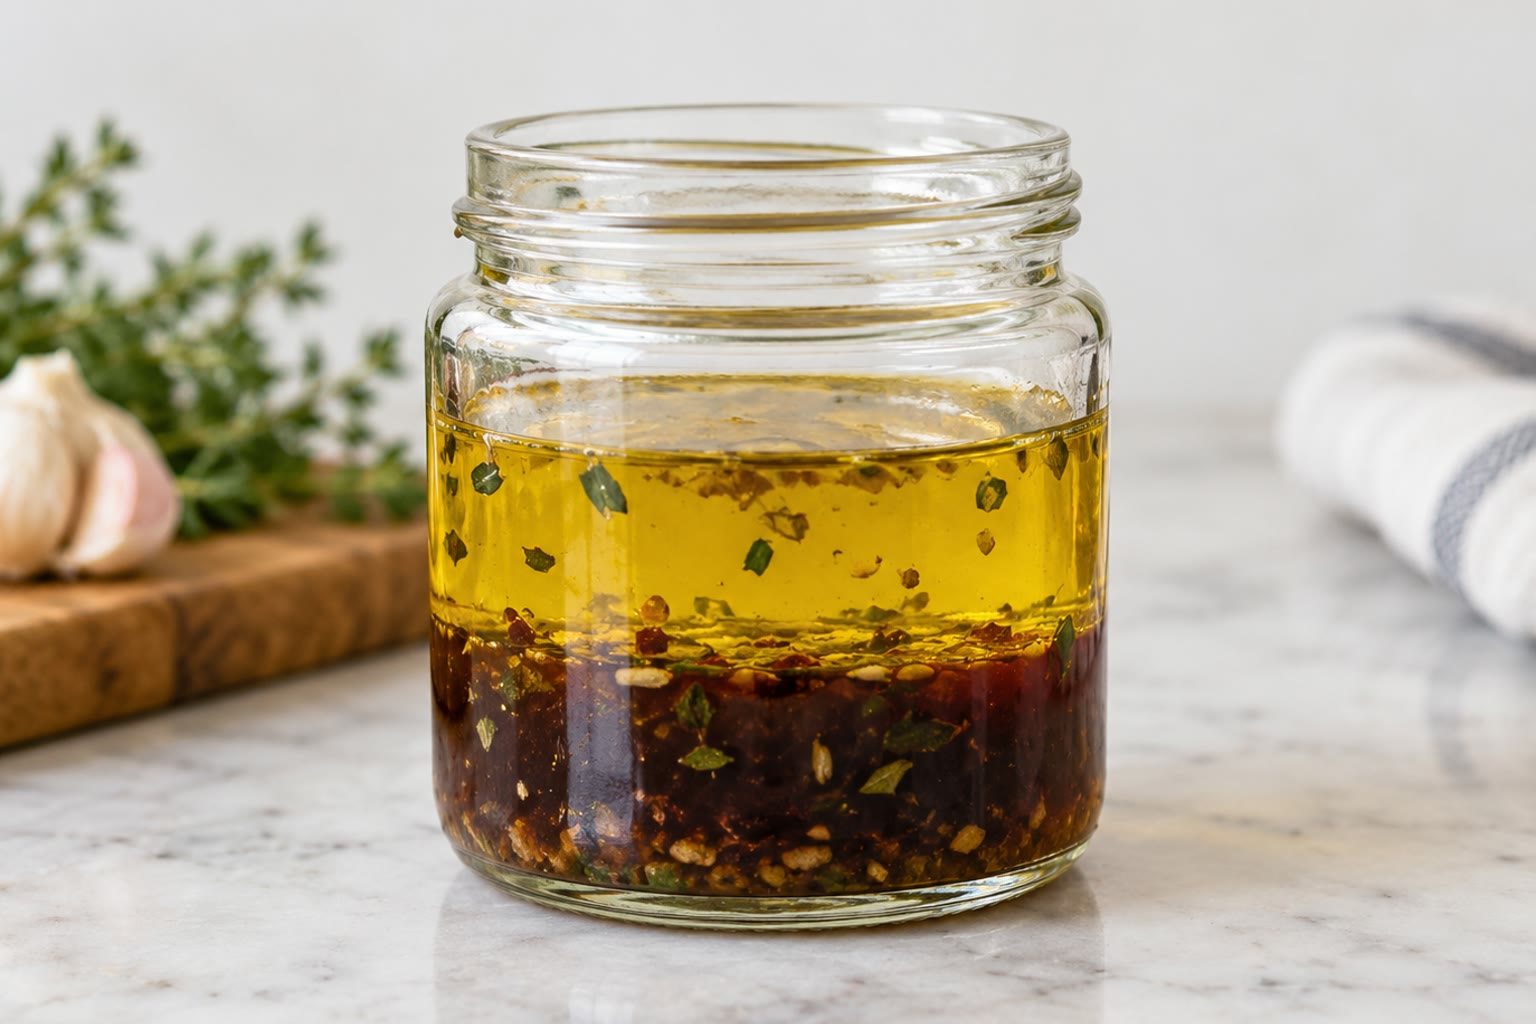
\includegraphics[width=0.45\linewidth]{images/book1/ai/g6-vinaigrette.jpg}

{\small Salad dressing: oil and vinegar are \omterm{def:g6:solutions-and-solubility:miscible}{immiscible}.}
\end{omfigure}

\section{Gases dissolve too}

\begin{proposition}[Dissolved gases]\label{prop:g6:solutions-and-solubility:gases}
Gases \omterm{def:g2:mixing-and-dissolving:dissolve}{dissolve} in water, a little. Sparkling drinks are made by
dissolving carbon dioxide in them under pressure in a closed bottle;
when the bottle is opened, part of the gas comes back out as bubbles.
Water in contact with \omterm{def:g4:air-a-mixture-of-gases:air}{air} holds some dissolved oxygen, which fish take
in through their gills. A gas \omterm{def:g2:mixing-and-dissolving:dissolve}{dissolves} less in warm water than in cold
water: a warm sparkling drink goes flat faster.
\end{proposition}

\begin{example}[Oceans and carbon dioxide]\label{ex:g6:solutions-and-solubility:oceans}
The oceans are in contact with the \omterm{def:g4:air-a-mixture-of-gases:air}{air} over two thirds of the Earth's
surface. Carbon dioxide of the \omterm{def:g4:air-a-mixture-of-gases:air}{air} \omterm{def:g2:mixing-and-dissolving:dissolve}{dissolves} in them, so the oceans take
up part of the carbon dioxide that people release into the \omterm{def:g4:air-a-mixture-of-gases:air}{air}.
\end{example}

\begin{omfigure}
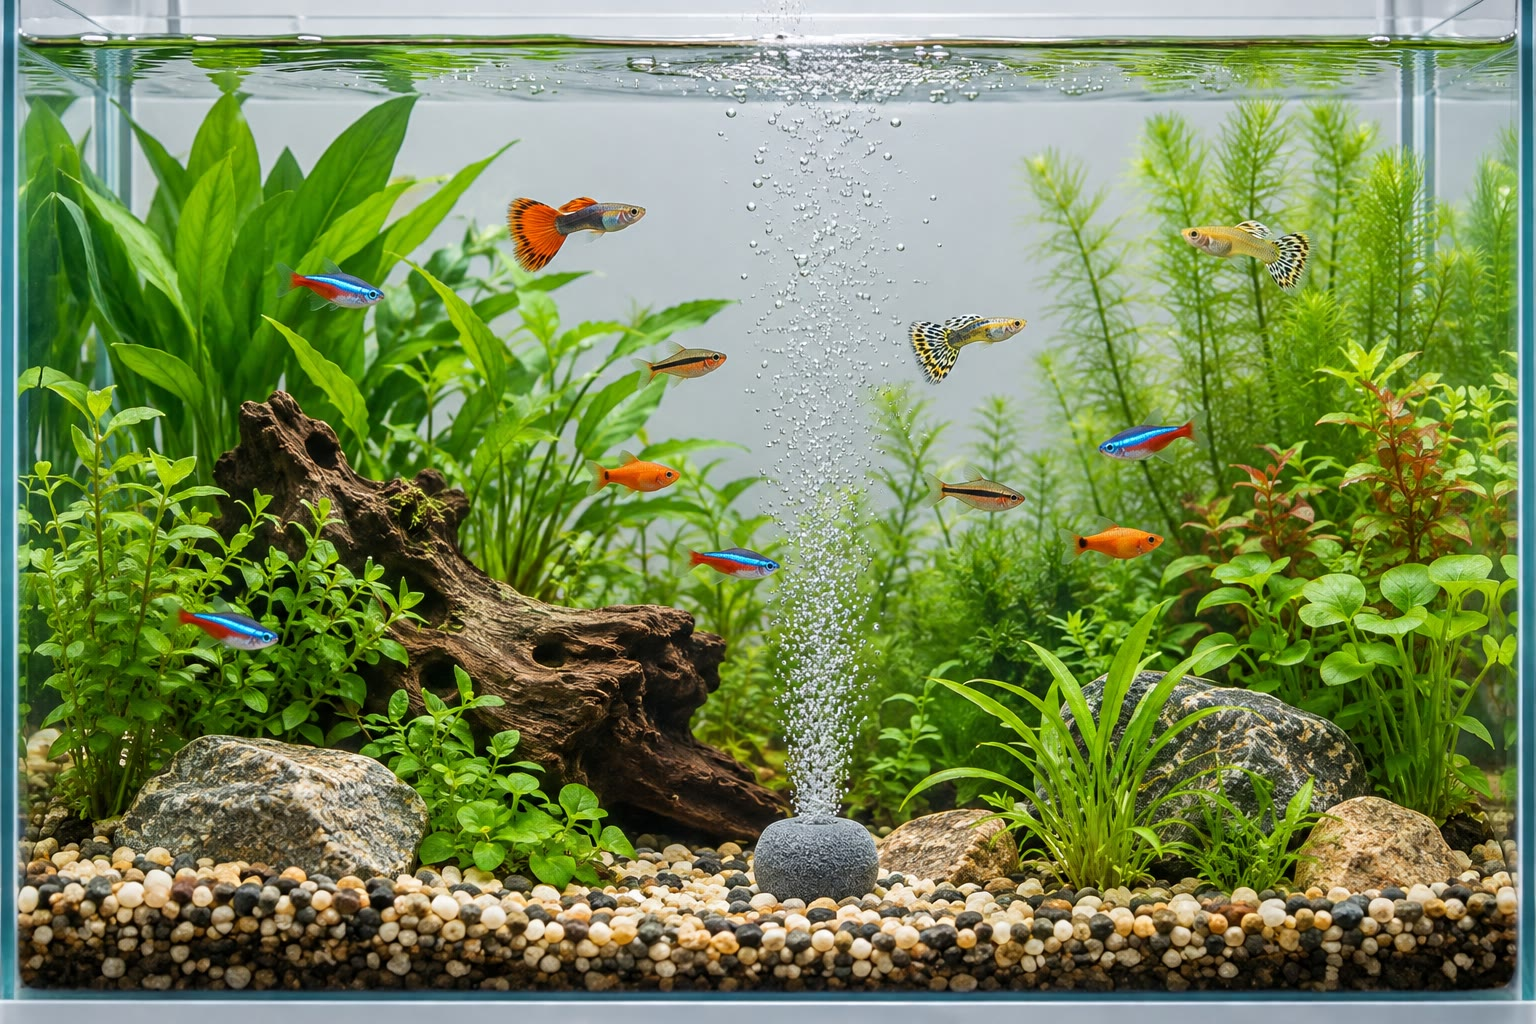
\includegraphics[width=0.5\linewidth]{images/book1/ai/g6-fish-tank.jpg}

{\small An aquarium: the \omterm{def:g4:air-a-mixture-of-gases:air}{air} bubbles keep the water supplied with
dissolved oxygen for the fish.}
\end{omfigure}

\section{Exercises}

\begin{exercise}[$\star$]\label{exo:g6:solutions-and-solubility:1}
In sugar water, name the \omterm{def:g6:solutions-and-solubility:solute}{solute} and the \omterm{def:g6:solutions-and-solubility:solute}{solvent}. Is it an \omterm{def:g6:solutions-and-solubility:solute}{aqueous
solution}?
\end{exercise}

\begin{exercise}[$\star$]\label{exo:g6:solutions-and-solubility:2}
What is a \omterm{def:g6:solutions-and-solubility:saturated}{saturated solution}? How can you see that a solution is
saturated?
\end{exercise}

\begin{exercise}[$\star$]\label{exo:g6:solutions-and-solubility:3}
\qty{20}{g} of salt are dissolved in \qty{250}{g} of water. What is the
mass of the solution?
\end{exercise}

\begin{exercise}[$\star$]\label{exo:g6:solutions-and-solubility:4}
\omterm{def:g6:solutions-and-solubility:miscible}{Miscible} or \omterm{def:g6:solutions-and-solubility:miscible}{immiscible} with water: ethanol, cooking oil, vinegar?
\end{exercise}

\begin{exercise}[$\star$]\label{exo:g6:solutions-and-solubility:5}
Name the \omterm{def:g6:solutions-and-solubility:solute}{solvent} of nail-varnish remover and give the meaning of its two
pictograms.
\end{exercise}

\begin{exercise}[$\star\star$]\label{exo:g6:solutions-and-solubility:6}
Using the \omterm{def:g6:solutions-and-solubility:solubility}{solubility} of salt, find the largest mass of salt that
\qty{500}{g} of water can \omterm{def:g2:mixing-and-dissolving:dissolve}{dissolve} at \qty{25}{\celsius}.
\end{exercise}

\begin{exercise}[$\star\star$]\label{exo:g6:solutions-and-solubility:7}
\qty{80}{g} of salt are stirred into \qty{200}{g} of water at
\qty{25}{\celsius}. Does it all \omterm{def:g2:mixing-and-dissolving:dissolve}{dissolve}? If not, what mass stays at the
bottom?
\end{exercise}

\begin{exercise}[$\star\star$]\label{exo:g6:solutions-and-solubility:8}
\qty{25}{g} of sugar are dissolved in \qty{225}{g} of water. What
percentage of the mass of the solution is sugar?
\end{exercise}

\begin{exercise}[$\star\star$]\label{exo:g6:solutions-and-solubility:9}
Look at the figure of the three beakers of salt water. In which beaker
could more salt still \omterm{def:g2:mixing-and-dissolving:dissolve}{dissolve}?
\end{exercise}

\begin{exercise}[$\star\star$]\label{exo:g6:solutions-and-solubility:10}
Why does a bottle of sparkling water fizz when it is opened, and not
before?
\end{exercise}

\begin{exercise}[$\star\star\star$]\label{exo:g6:solutions-and-solubility:11}
A litre of water can \omterm{def:g2:mixing-and-dissolving:dissolve}{dissolve} about \qty{2000}{g} of sugar but only
about \qty{0.04}{g} of oxygen. How many times more sugar than oxygen is
that?
\end{exercise}

\begin{exercise}[$\star\star\star$]\label{exo:g6:solutions-and-solubility:12}
In summer, the water of a pond warms up and fish come up to the surface
to gulp \omterm{def:g4:air-a-mixture-of-gases:air}{air}. Use this chapter to explain why.
\end{exercise}

\section{Problem: The Cheese-Maker's Brine}

\begin{problem}[{Weekend problem --- a bath of saturated salt water for
cheeses, and what the summer heat does to it}]
\label{pb:g6:solutions-and-solubility:1}
% ledger: sol:NaCl (360 g per kg of water; 1 L of water taken as 1 kg)
Many cheeses are soaked for a few hours in a bath of brine: water
saturated with salt. A cheese-maker fills a tank with \qty{20}{L} of
water (\qty{20}{kg}) and adds salt until some stays undissolved at the
bottom. Take the \omterm{def:g6:solutions-and-solubility:solubility}{solubility} of salt as \qty{360}{g} per kilogram of
water.

\medskip
\noindent\textbf{Part I --- Words.}
\begin{enumerate}
  \item In the brine, which is the \omterm{def:g6:solutions-and-solubility:solute}{solute} and which the \omterm{def:g6:solutions-and-solubility:solute}{solvent}?
  \item What does ``saturated'' mean for the brine?
  \item Why does the cheese-maker add salt until a little stays at the
        bottom?
\end{enumerate}

\medskip
\noindent\textbf{Part II --- Making the brine.}
\begin{enumerate}[resume]
  \item What mass of salt \omterm{def:g2:mixing-and-dissolving:dissolve}{dissolves} in the \qty{20}{kg} of water?
  \item What is the mass of the brine (without the undissolved salt)?
  \item What percentage of the mass of the brine is salt? Round to the
        nearest whole number.
  \item One day only \qty{5}{kg} of salt are added. Is the brine
        saturated? How much more salt could it \omterm{def:g2:mixing-and-dissolving:dissolve}{dissolve}?
\end{enumerate}

\medskip
\noindent\textbf{Part III --- A hot summer.}
During a hot week, \qty{5}{L} (\qty{5}{kg}) of water evaporate from the
saturated brine of Part II, and no salt is lost.
\begin{enumerate}[resume]
  \item How much water is left in the tank?
  \item What mass of salt can this water still hold dissolved?
  \item What happens to the salt that the remaining water cannot hold?
  \item How can the cheese-maker see, by looking, that this has
        happened?
  \item Compute the mass of salt that has crystallised at the bottom of
        the tank.
\end{enumerate}
\end{problem}
